\chapter{Introduzione}
\chaptermark{Introduzione}
\label{chap:introduction}

Il cloud computing è un modello di erogazione di servizi che consente di gestire l'infrastruttura informatica necessaria
per rendere disponibili applicazioni, dati e servizi online in modo rapido, efficiente e flessibile. Grazie al cloud
computing, le risorse informatiche come server, storage e software possono essere facilmente scalate per rispondere alle
esigenze delle organizzazioni e degli utenti finali, consentendo un accesso sicuro e veloce ai servizi e alle
applicazioni da qualsiasi dispositivo connesso a Internet. La rapidità e velocità con cui il cloud computing eroga
questi servizi è data dalle tecnologie che lo compongono. \\
In questo contesto andremo a discutere di una emergente tecnologia, chiamata \textbf{WASI (WebAssembly System
Interface)}\footnote{\url{https://wasi.dev/}} e come questa possa essere considerata la terza ondata del cloud
computing\cite{cloudcomputing-thirdwave}. Grazie a WASI, è possibile eseguire applicazioni in un ambiente isolato e
sicuro, senza la necessità di dover conoscere il sistema operativo sottostante. È stato progettato per essere altamente
portabile, consentendo alle applicazioni di essere eseguite in modo efficiente su qualsiasi piattaforma. \\
Nasce e si sviluppa sopra ad una tecnologia già esistente: \textbf{WebAssembly} (o \textbf{Wasm}). Quest'ultima è
un'innovativa tecnologia nata con l'obiettivo di migliorare le prestazioni delle applicazioni web \textbf{sul browser}.
È stata progettata con l'intento di superare le limitazioni poste da Javascript. In particolare, si propone di essere
veloce, efficiente e portabile, oltre che retro-compatibile con le tecnologie già esistenti. Va notato che WebAssembly
non è pensato per sostituire JavaScript, ma piuttosto per migliorare le aree in cui quest'ultimo presenta alcune lacune:
come il rendering 3D, il video editing, giochi in-browser e così via. \\\\
WASI eredita tutte queste caratteristiche da Wasm e le utilizza per lo sviluppo di applicazioni \textbf{al di fuori} dei
browser. \\\\
Di seguito andremo ad approfondire WASI ed esporremo come rappresenti una tecnologia estremamente promettente per il
futuro nell'ambito del cloud computing in particolare, sebbene sia ancora in fase di sviluppo e di adozione.

\clearpage

\section{Un focus su WebAssembly}
\label{sec:webassembly}
Tradizionalmente, l'unico linguaggio utilizzabile all'interno dei browser era JavaScript, perfetto per la creazione di
interfacce utente ma non per operazioni che richiedono una complessità maggiore. WebAssembly è stato progettato per
essere un formato di esecuzione più efficiente, veloce e sicuro rispetto a JavaScript, da usare in combinazione con
esso\cite{webassembly-concepts}. \\
In sintesi, WebAssembly è un formato binario (.wasm) progettato per essere eseguito da una macchina virtuale integrata
all'interno dei browser. Grazie alla sua natura binaria, è possibile utilizzare diversi linguaggi di programmazione,
come C, C++ e Rust, che supportano questo formato. \\
Ogni file .wasm contiene un \textbf{modulo}, che può essere visto come un'unità di codice autonomo, composto da
funzioni, dati e altre risorse. Il modulo viene eseguito all'interno della macchina virtuale del browser in modalità
sandboxed, che garantisce l'isolamento e la sicurezza dell'esecuzione. \\
Ogni rappresentazione binaria possiede anche una duale rappresentazione testuale chiamata \textbf{WebAssembly Text
Format (.wat)}. Questo formato ha una sintassi simile ai linguaggi Assembly, il che lo rende più leggibile per gli
esseri umani rispetto al formato binario. Un file .wat è costituito da una serie di istruzioni che definiscono la
struttura del modulo organizzate in sezioni. \\
Il vantaggio di avere una rappresentazione testuale come il formato .wat è che può aiutare gli sviluppatori a
comprendere meglio la struttura e il funzionamento dei moduli, anche se non sono esperti nel linguaggio Assembly o
nell'architettura della CPU.

\begin{figure}[h]
    \centering
    \captionsetup{justification=centering}
    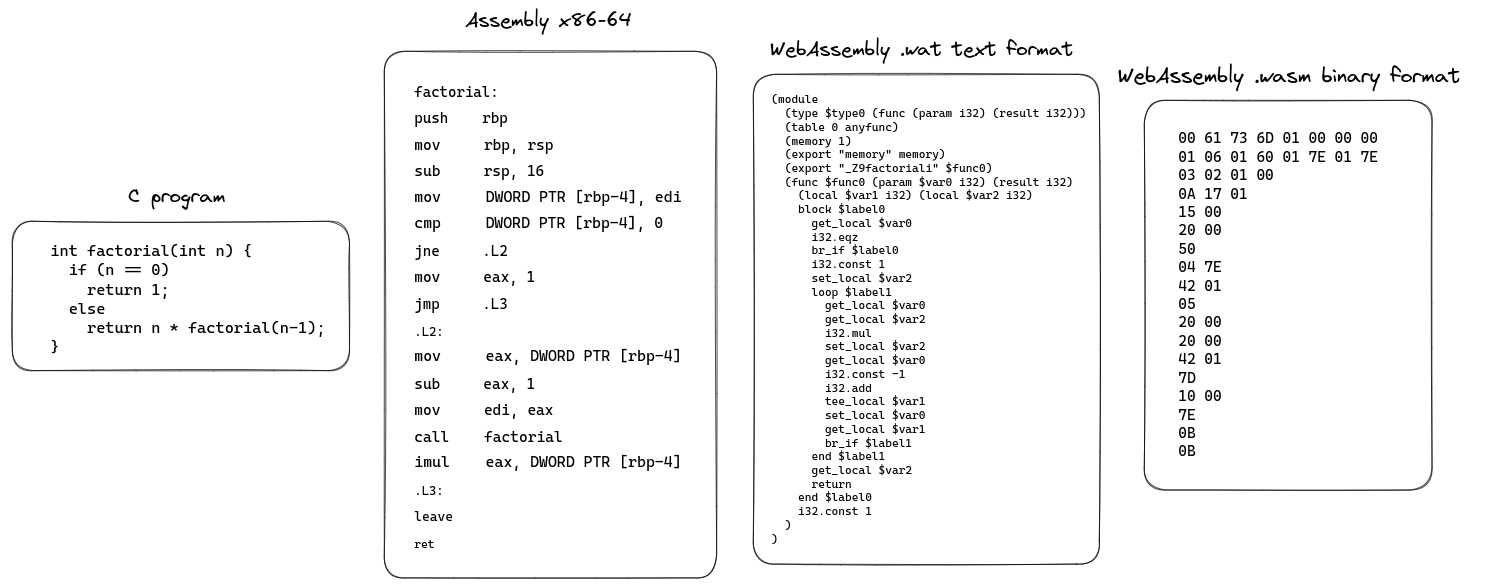
\includegraphics[width=15cm]{./chapters/1.introduction/images/3.source_code_wat_wasm.png}
    \label{source_code_wat_wasm}
    \caption{Esempio di una funzione compilata nel modo 'tradizionale', in .wasm e la sua rappresentazione in .wat}
\end{figure}

Come noto, i linguaggi Assembly tradizionali sono strettamente legati all'architettura della CPU sottostante. Ciò
significa che ogni programma scritto in Assembly è vincolato alla specifica architettura su cui deve essere eseguito.
Pertanto, per rendere un'applicazione compatibile ed eseguibile su diverse macchine, è necessario compilarla per le
diverse architetture che si vogliono supportare. Nel corso degli anni, gli sviluppatori hanno cercato di risolvere
questo problema attraverso diverse soluzioni. Ad esempio, il linguaggio Java ha introdotto il motto "Write once, run
anywhere". Wasm può essere considerato come una soluzione simile, ma con un vantaggio fondamentale: mentre Java richiede
agli sviluppatori di scrivere codice nel linguaggio Java o in linguaggi compatibili con la Java Virtual Machine, per
poterlo eseguire su qualsiasi piattaforma, Wasm consente di utilizzare qualsiasi linguaggio di programmazione
compilabile in formato .wasm e il risultante codice prodotto può essere eseguito su tutti i browser compatibili. \\
Tuttavia, gli sviluppatori non si sono limitati ad utilizzare Wasm solo all'interno dei browser. Anche per lo sviluppo
di applicazioni tradizionali, Wasm sta diventando sempre più popolare. In questo contesto, WASI svolge un ruolo
cruciale. Mentre all'interno del browser Wasm non ha bisogno di comunicare con il sistema operativo, poiché il browser
funge da intermediario, al di fuori di esso, la situazione è diversa. Qui, l'applicazione deve comunicare con il
filesystem, creare connessioni di rete, eseguire codice in parallelo e così via, e farlo in modo sicuro, isolando
l'applicazione dal sistema operativo sottostante e garantendo che non possa interferire con altri processi o con la
memoria del sistema. \\
WASI affronta queste sfide fornendo un insieme di interfacce standardizzate, una \textbf{system interface}, tra le
applicazioni Wasm e l'ambiente di esecuzione sottostante.
\clearpage
\section{Cos'è una System Interface?}
Normalmente, le applicazioni non si interfacciano direttamente con le risorse del sistema, ma attraverso il sistema
operativo, il cui nucleo è il kernel, che media l'accesso alle risorse. Ciò è necessario per evitare accessi
indiscriminati, che potrebbero causare instabilità e problemi di sicurezza. Per questo motivo, il sistema operativo
organizza la protezione in strati a livelli crescenti di privilegi. Ogni programma viene eseguito in "user mode" e se
vuole eseguire operazioni privilegiate, deve chiedere al kernel di farlo attraverso le \textbf{system call}, che
eseguono i controlli necessari prima di permettere l'operazione. \\
Per semplificare l'accesso alle risorse del sistema, molti linguaggi di programmazione forniscono una libreria standard
che definisce un'interfaccia comune, chiamata system interface, indipendente dal sistema operativo sottostante. Ciò
significa che gli sviluppatori non devono preoccuparsi dell'implementazione specifica del sistema operativo, poiché
possono utilizzare l'interfaccia fornita dal linguaggio di programmazione. Sarà il compilatore a scegliere
l'implementazione corretta dell'interfaccia in base al sistema operativo in cui viene eseguita l'applicazione.
\begin{figure}[h]
    \centering
    \captionsetup{justification=centering}
    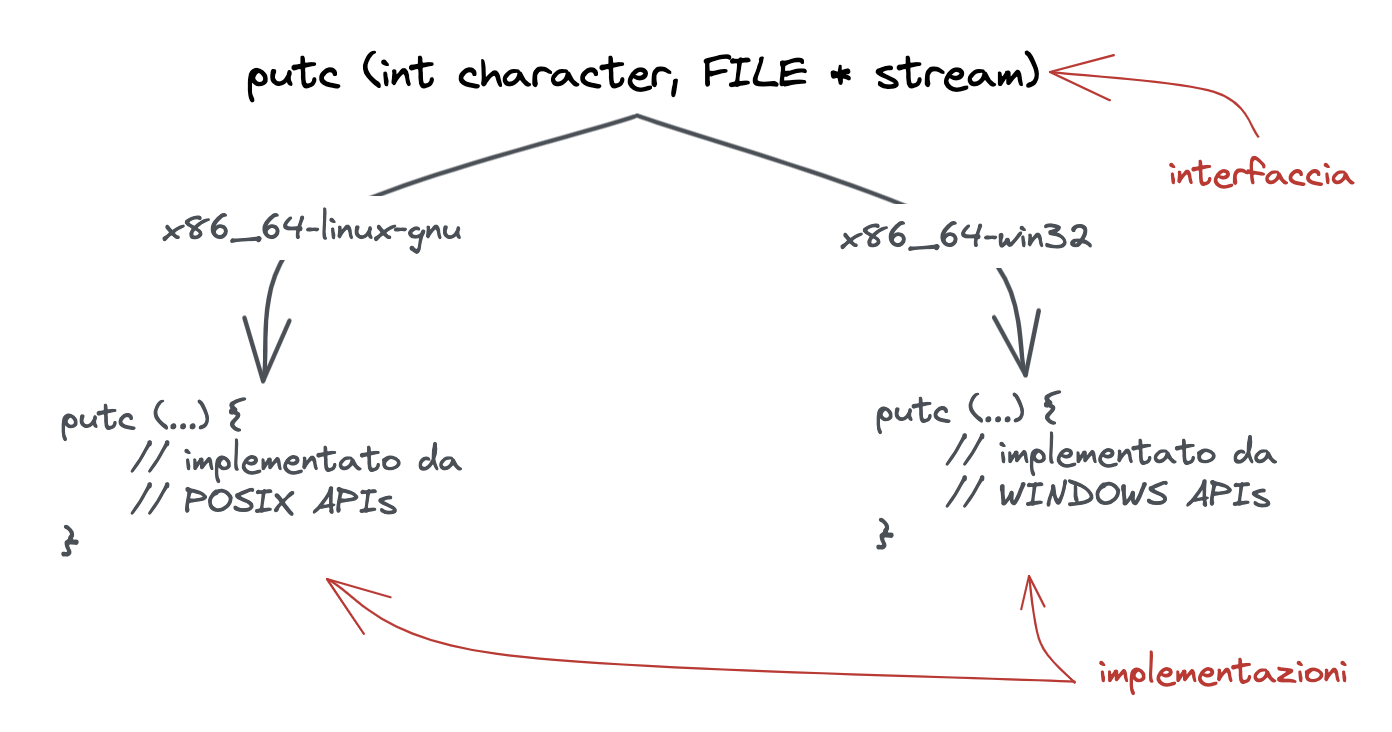
\includegraphics[width=15cm]{./chapters/1.introduction/images/5.system-interface-api-to-impl.png}
    \label{system-interface-api-to-impl}
    \caption{System Interface: Dall'API alla sua implementazione}
\end{figure}

Con WebAssembly, invece, è necessario definire un'interfaccia per un sistema operativo concettuale e un runtime che la
implementi, poiché non si conosce a priori il sistema operativo su cui verrà eseguito il modulo .wasm.
\begin{figure}[H]
    \centering
    \captionsetup{justification=centering}
    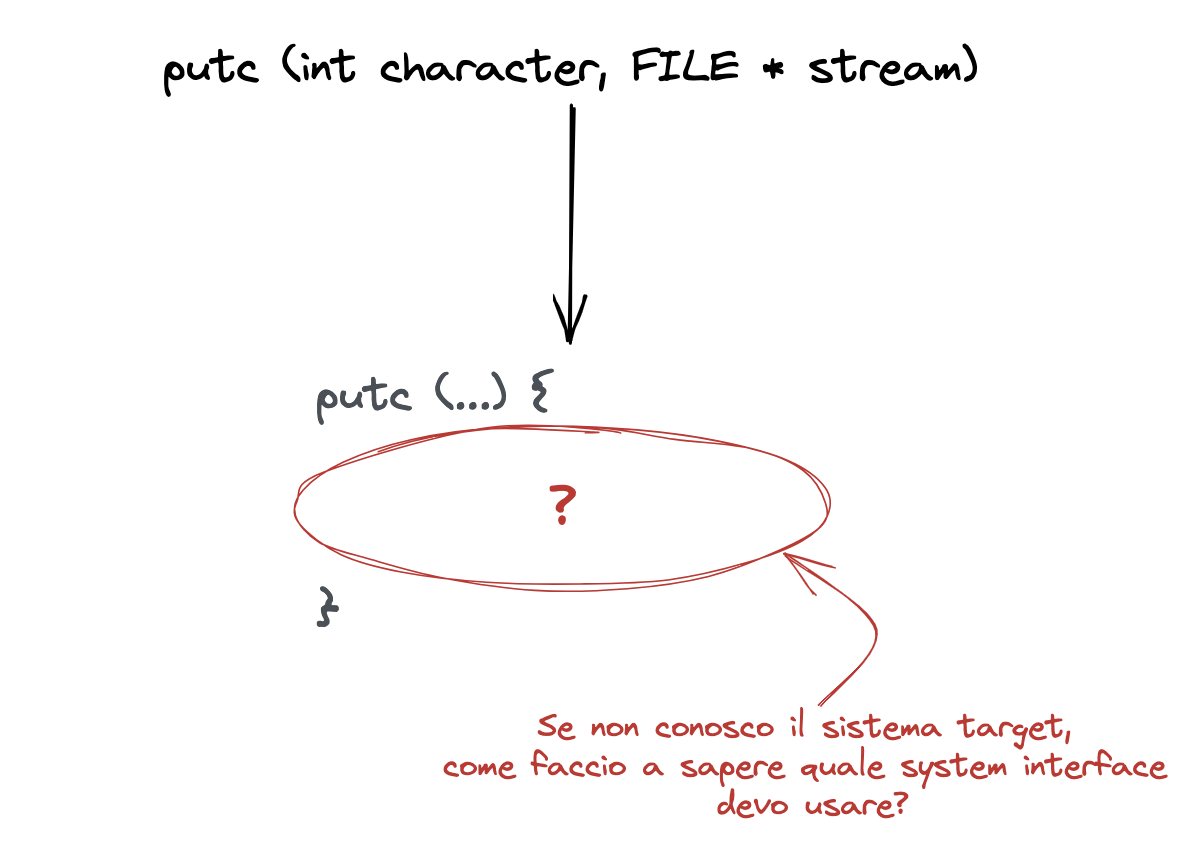
\includegraphics[width=15cm]{./chapters/1.introduction/images/5a.wasi_sys_interface.png}
    \label{system-interface-conceptual-sys}
    \caption{Una System Interface per un sistema operativo concettuale}
\end{figure}
Questa interfaccia deve essere poi implementata dai runtime capaci di eseguire effettivamente i moduli wasm.

\section{Il valore aggiunto}
Cosa differenzia Wasm e WASI da altri linguaggi di programmazione e tecniche di sviluppo? Wasm è stato concepito tenendo
a mente le necessità del web, ogni runtime browser deve quindi soddisfare i seguenti requisiti:

\begin{itemize}
    \item \textbf{Sicurezza}: dato che il browser esegue codice proveniente da Internet, è essenziale che il codice
    eseguito sia controllato e limitato affinché non possa fare ciò che vuole.
    \item \textbf{Dimensioni Ridotte}: poiché la larghezza di banda è una limitazione costante su Internet, il codice
    scaricato deve essere il più piccolo possibile, occupando al più pochi megabyte di dati.
    \item \textbf{Caricamento ed esecuzioni veloci}: se una pagina web non risponde entro pochissimo tempo (circa 3
    secondi\footnote{\url{https://www.thinkwithgoogle.com/consumer-insights/consumer-trends/mobile-site-load-time-statistics/}}),
    gli utenti la abbandonano.
    \item \textbf{Portabilità}: nell'era degli smartphone, tablet, dispositivi IoT, sensori e altre tecnologie
    eterogenee, è necessario garantire che la stessa applicazione possa essere eseguita su tutti i dispositivi, a
    prescindere dal sistema operativo e dall'architettura sottostante.
\end{itemize}

Si può notare come questi requisiti possono sicuramente essere un punto di forza anche al di fuori del browser. In
particolare, Wasm e WASI migliorano due aspetti molto importanti già ampiamente affrontati in letteratura: la
portabilità e la sicurezza.

\subsection{Portabilità}
I linguaggi tradizionali consentono di eseguire codice su diverse architetture, ma richiedono di essere compilati una
volta per ogni architettura di destinazione.
\begin{figure}[H]
    \centering
    \captionsetup{justification=centering}
    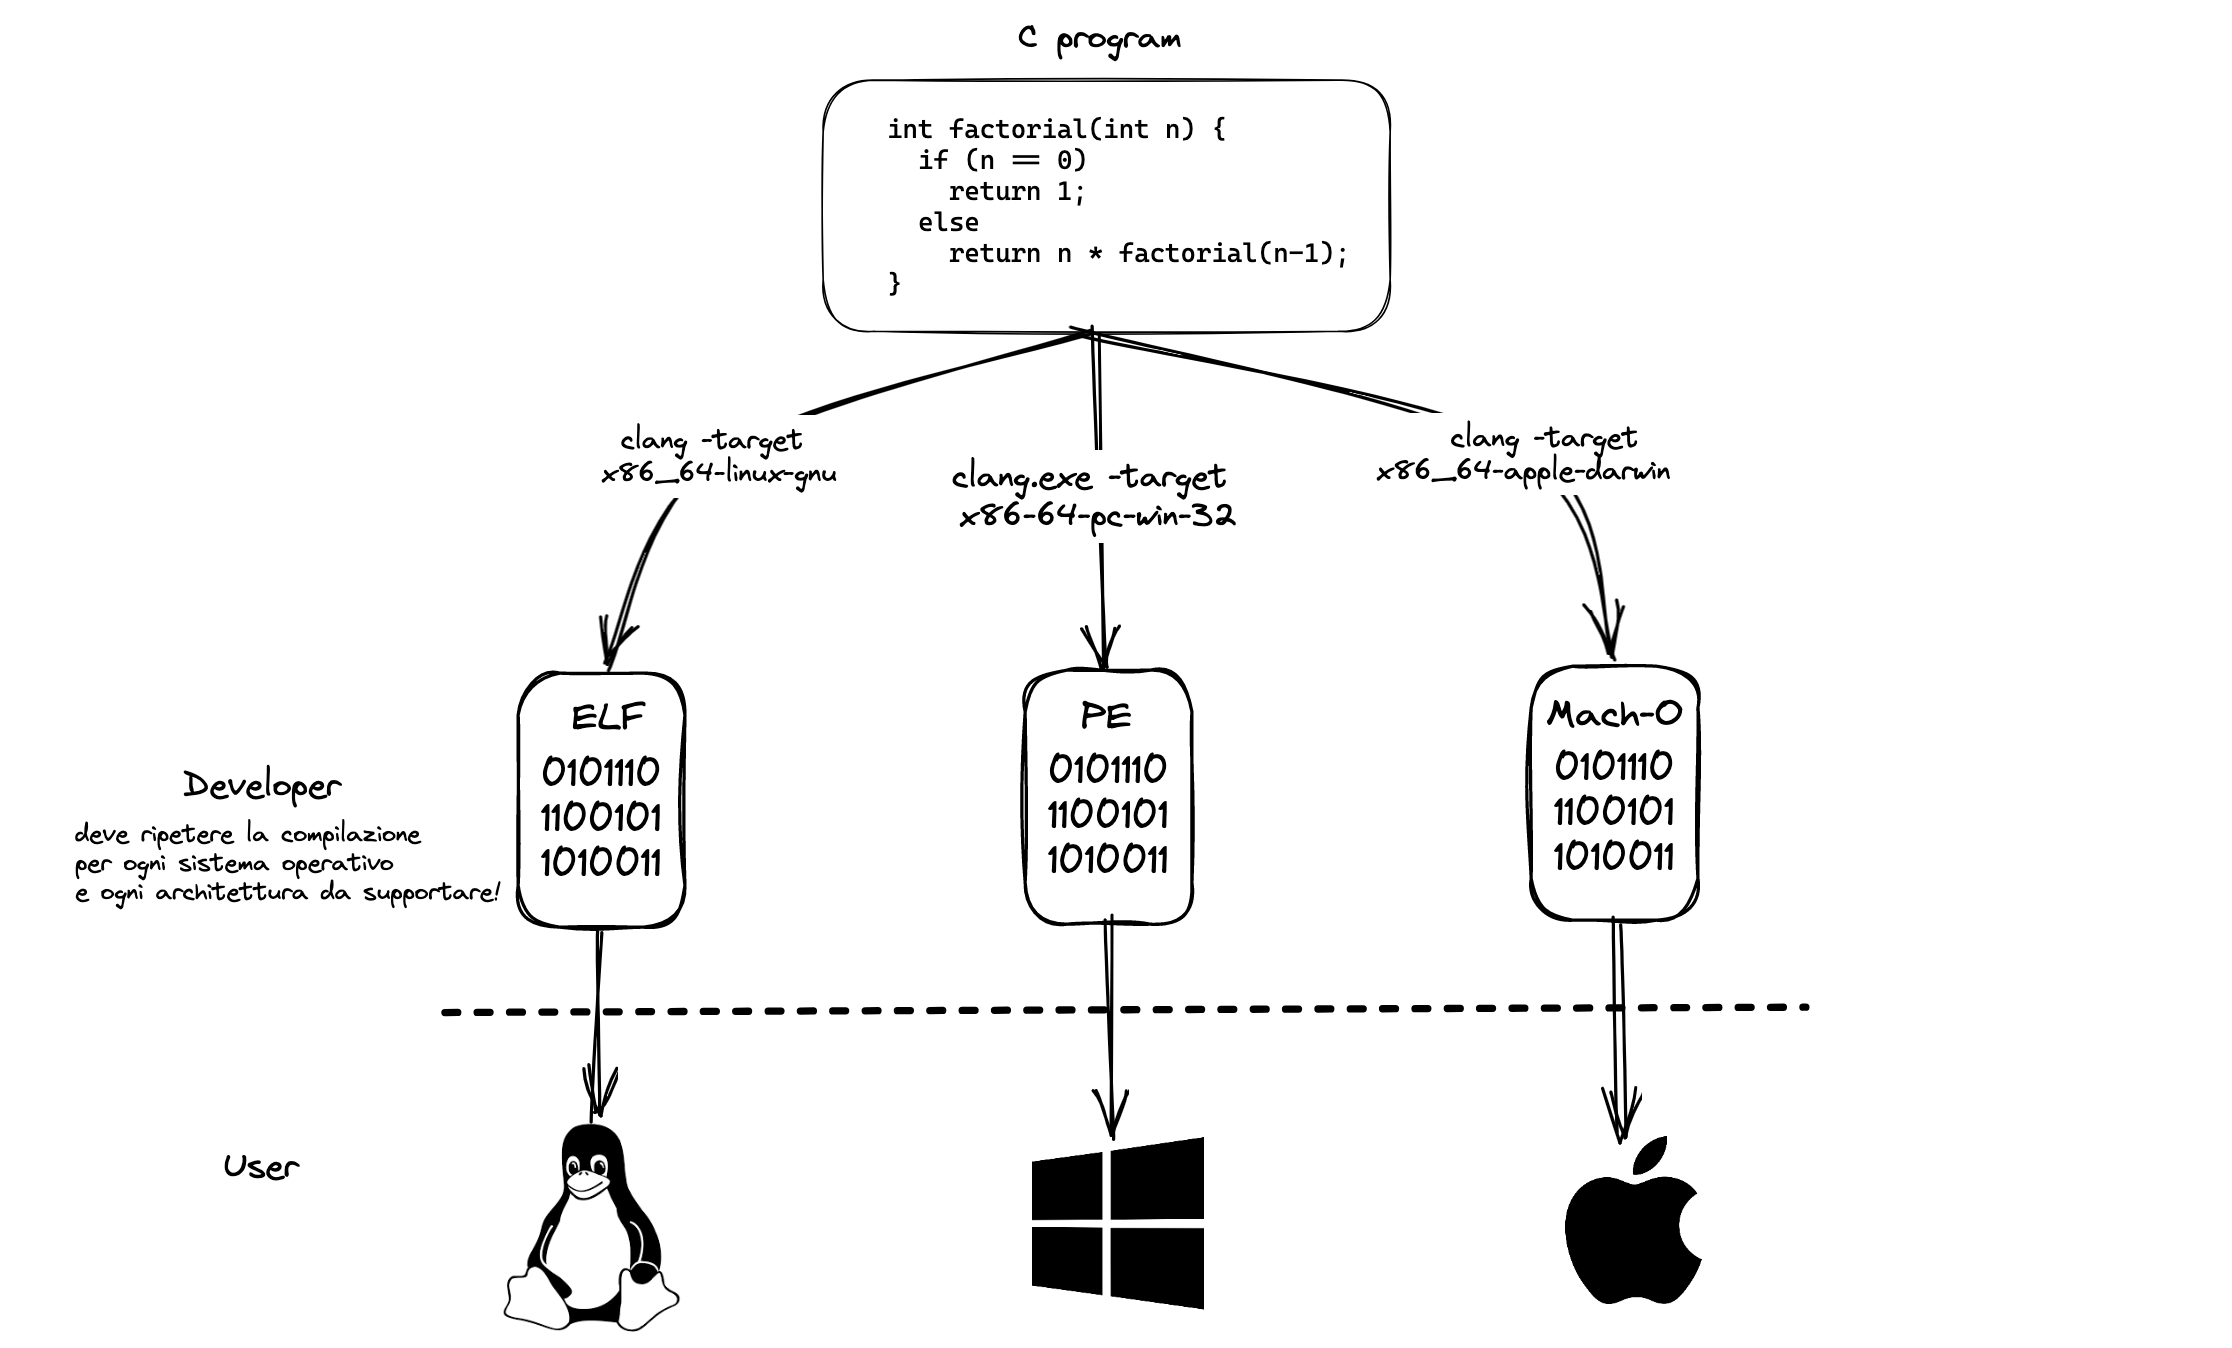
\includegraphics[width=15cm]{./chapters/1.introduction/images/6.c_compilation_portability.png}
    \label{traditional_programming_portability}
    \caption{Portabilità in senso tradizionale}
\end{figure}
Con Wasm e WASI, invece, la situazione è completamente diversa. Una volta compilata l'applicazione, è possibile
eseguirla su qualsiasi runtime in grado di gestire il codice Wasm. Questo approccio è noto come "Write once, run
anywhere”.
\begin{figure}[H]
    \centering
    \captionsetup{justification=centering}
    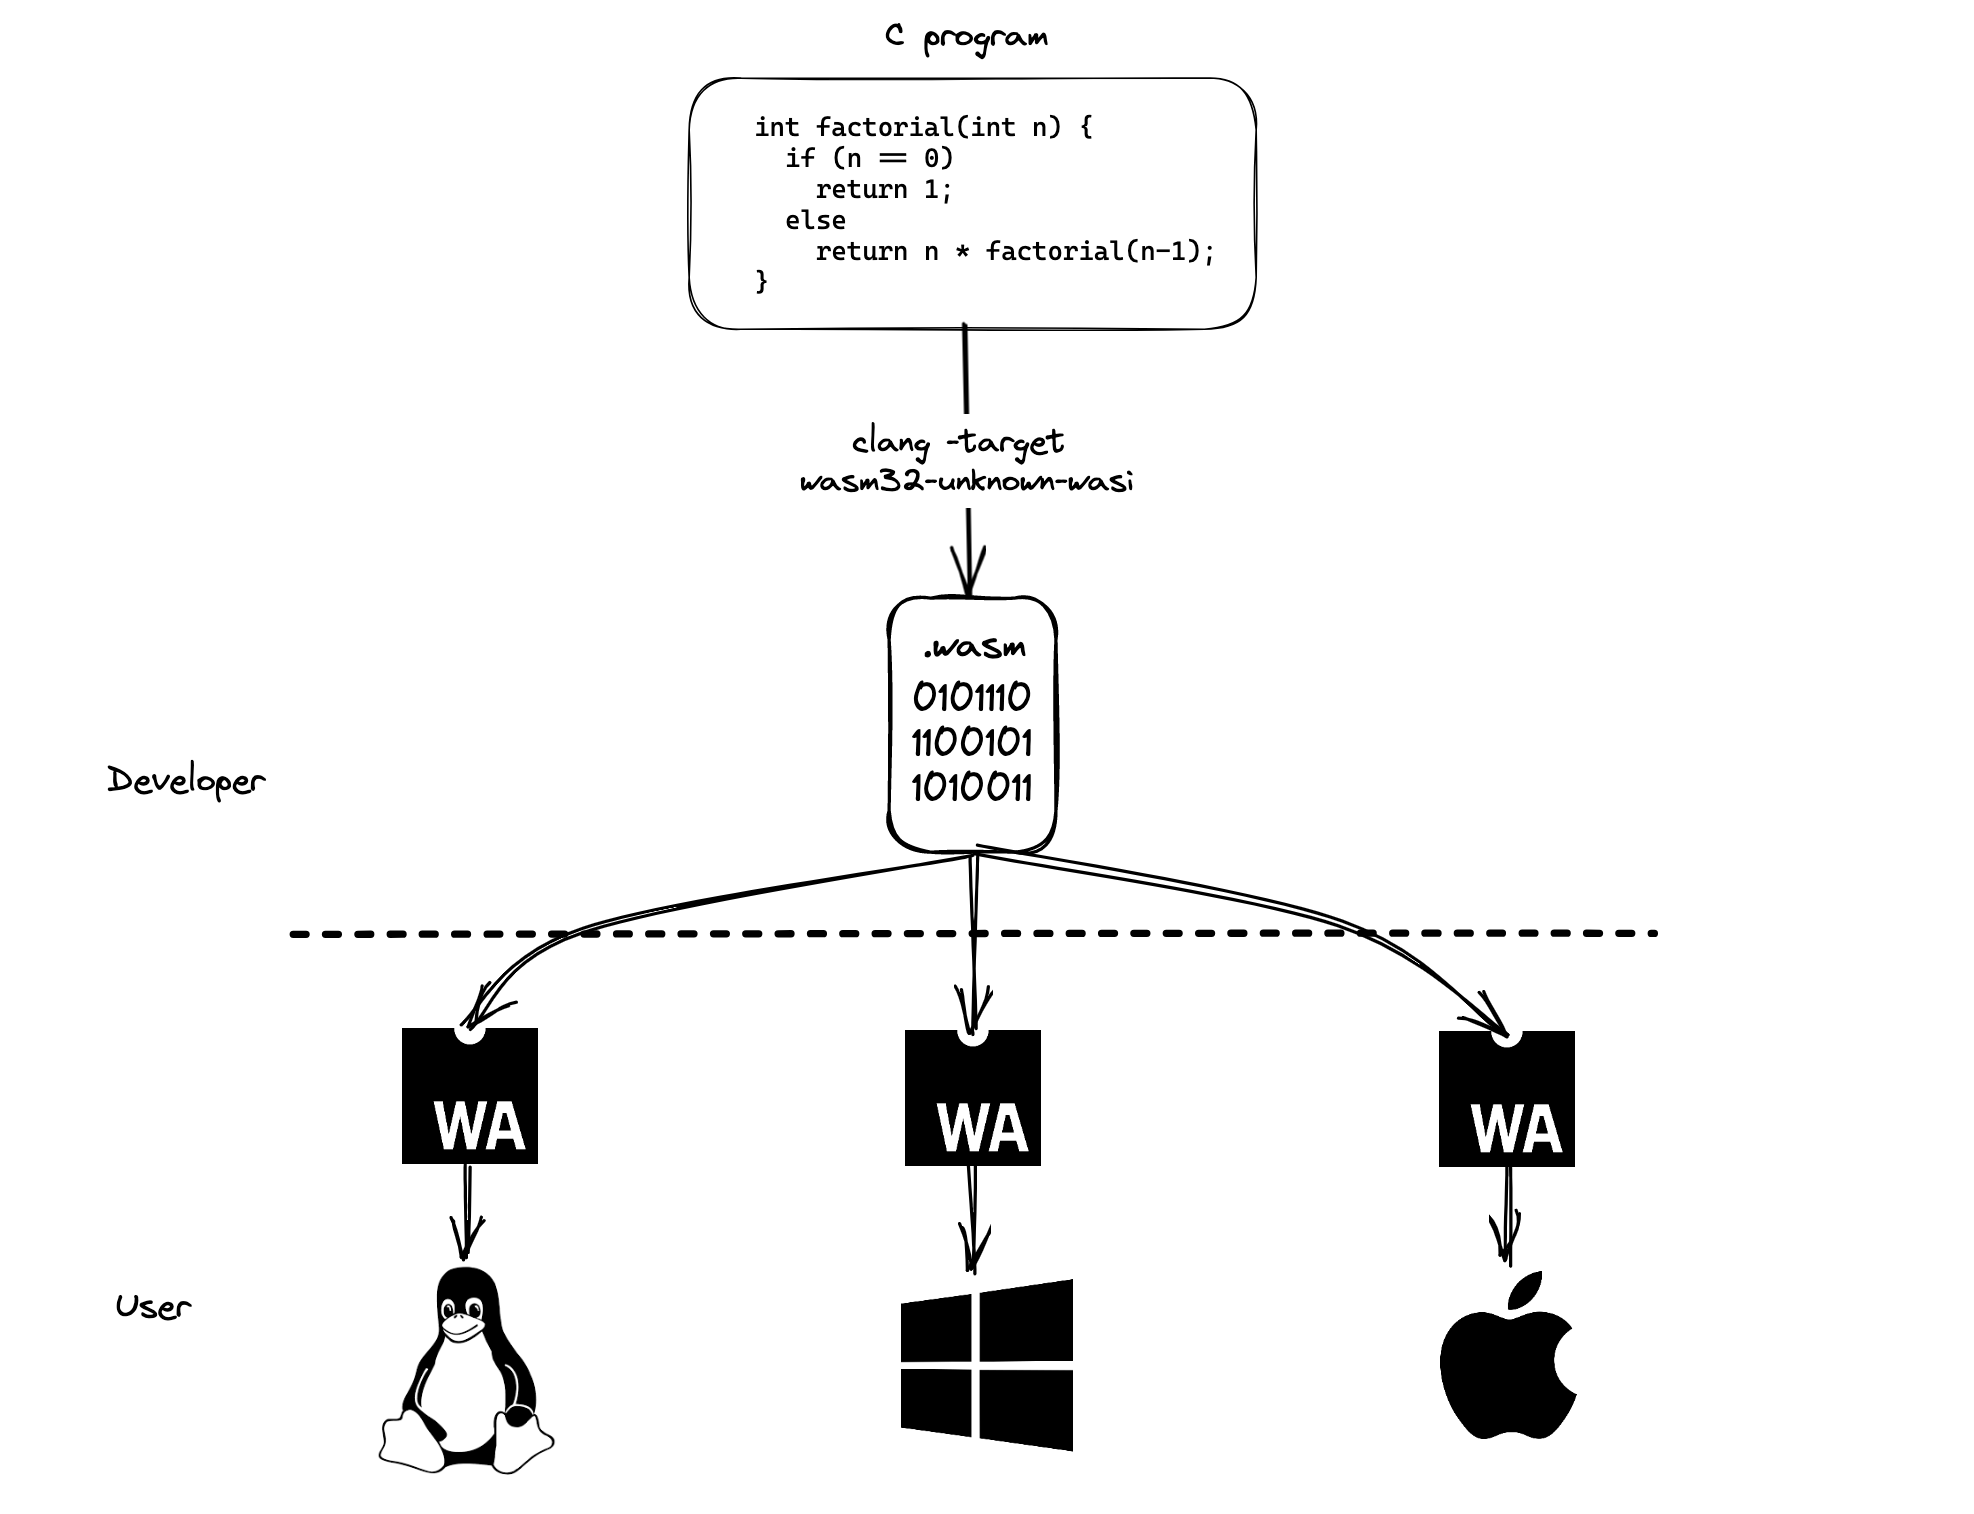
\includegraphics[width=15cm]{./chapters/1.introduction/images/6.wasm_compilation_portability.png}
    \label{wasm_wasi_programming_portability}
    \caption{Portabilità con Wasm e WASI}
\end{figure}
Si potrebbe obiettare che l'approccio di WebAssembly non rappresenta nulla di innovativo, dato che linguaggi
interpretati come Java hanno già affrontato questa problematica. Tuttavia, bisogna considerare che WebAssembly non è
legato a nessun linguaggio di programmazione specifico, ma rappresenta un formato binario generico indipendente. Al
contrario, il bytecode di Java (metalinguaggio simile al .wat di Wasm) è strettamente legato al linguaggio stesso e
rappresenta quindi un ostacolo alla portabilità del codice. Questo problema riguarda anche altri linguaggi interpretati,
prendiamo come altro esempio Python, che utilizza un approccio simile generando il bytecode prima di poter eseguire il
codice sorgente nella sua apposita macchina virtuale. Anche in questo caso, il bytecode di Python è strettamente legato
al linguaggio stesso, impedendo una piena portabilità del codice. \\In secondo luogo Wasm non dipende da una azienda
privata, è uno standard del World Wide Web Consortium
(W3C)\footnote{\url{https://www.w3.org/2019/12/pressrelease-wasm-rec.html.en}} e quindi non segue una sola linea di
pensiero per la sua sua evoluzione. \\
Infine, c'è da considerare come WASI affronta in maniera diversa dagli altri un'altro aspetto fondamentale: la
sicurezza.

\subsection{Sicurezza}
Abbiamo precedentemente descritto come le applicazioni accedono alle risorse del sistema tramite le system call,
richiedendo al kernel le operazioni desiderate. Tuttavia, questo modello non garantisce una protezione completa da
eventuali minacce, poiché l'accesso alle risorse viene concesso in base ai permessi dell'utente che sta eseguendo
l'applicazione. Questo approccio, nato agli albori dei sistemi operativi, si adattava bene alle esigenze dell'epoca,
quando le applicazioni venivano controllate ed installate dagli amministratori di sistema. Tuttavia, con la diffusione
di internet, molte applicazioni, la cui origine non può sempre essere verificata con certezza, vengono eseguite sui
computer degli utenti finali. Questo comporta un elevato rischio di vulnerabilità e di compromissione della sicurezza
del sistema. Il codice Wasm, invece, viene eseguito in un ambiente isolato e controllato separato dal sistema operativo,
chiamato "sandbox". In questo ambiente, il codice non ha accesso diretto alle risorse del sistema e non può interagire
direttamente con il livello sottostante. Al contrario, deve passare attraverso l'host (il browser o il runtime Wasm) che
contiene le funzioni necessarie per farlo. Questo permette all'host di limitare ciò che un programma può fare a priori.
In altre parole, un'applicazione non viene eseguita con gli stessi privilegi dell'utente e quindi non può direttamente
invocare le system call. Questo modello si basa sul concetto di "capacità" che definisce ciò che un programma Wasm può
fare e sono definite prima dell'esecuzione dell'applicazione. Questo modello, noto come "capability-based model",
fornisce una maggiore sicurezza e limita il rischio di compromissione del sistema.

\section{Stato dell'arte}
Per poter cogliere appieno la direzione verso cui si stanno muovendo Wasm e WASI, è necessario considerare l'attuale
panorama tecnologico. 

\subsection{Chi supporta Wasm?}
Dal punto di vista di un linguaggio di programmazione, Wasm non è altro che un altro target di compilazione.
\begin{itemize}
    \item Per qualsiasi linguaggio compilato, l'ostacolo per l'esecuzione in un contesto WebAssembly è rappresentato
    dalla possibilità o meno di compilare i programmi nel formato binario Wasm.
    \item Per qualsiasi linguaggio di scripting, l'ostacolo per l'esecuzione in un contesto WebAssembly è la possibilità
    di compilare l'interprete in WebAssembly.
\end{itemize}

Fortunatamente, il supporto a WebAssembly sta crescendo rapidamente. Inizialmente, solo C/C++ e Rust erano in grado di
generare codice .wasm, ma ora sempre più linguaggi stanno iniziando a supportarlo. Di seguito è riportata una tabella
che riassume il supporto dei linguaggi più popolari\cite{most-popular-technologies-stack-overflow}. È divisa in tre
categorie: \textit{Browser} (supporto nativo nei browser) e in
\textit{ambiente WASI}.
\begin{table}[H]
    \centering
    \begin{tabular}{|l|l|l|l|l|}
    \hline
        \textbf{Linguaggio} & \textbf{Browser} & \textbf{WASI} \\ \hline
        Javascript & Wip & Wip  \\ \hline
        Python & Wip & Sì  \\ \hline
        Java & Sì & No  \\ \hline
        PHP & Sì & Sì  \\ \hline
        C\# e .NET & Sì & Sì  \\ \hline
        Ruby & Sì & Sì  \\ \hline
        Swift & Sì & Sì  \\ \hline
        Typescript & No & No  \\ \hline
        C/C++ & Sì & Sì  \\ \hline
        Rust & Sì & Sì  \\ \hline
        Go & Sì & Sì  \\ \hline
        Kotlin & Sì & Wip  \\ \hline
    \end{tabular}
    \caption{Supporto a Wasm}
\end{table}

\subsection{A che punto è lo standard}
Nel caso di WASI, ogni nuova interfaccia inserita nello standard, nota come WASI API, segue un rigoroso percorso diviso
in sei fasi\footnote{\url{https://github.com/WebAssembly/meetings/blob/main/process/phases.md}} prima di essere
standardizzata:
\begin{itemize}
    \item \textbf{Pre-Proposal}: presentazione dell'idea iniziale e valutazione della sua fattibilità e rilevanza dalla
    comunità degli sviluppatori.
    \item \textbf{Feature Proposal}: presentazione dettagliata di una nuova funzionalità o modifica all'API esistente,
    valutata dalla comunità degli sviluppatori.
    \item \textbf{Spec Text Available}: scrittura del testo di specifica proposto con la descrizione dettagliata di come
    la nuova funzionalità o modifica dell'API dovrebbe essere implementata.
    \item \textbf{Implementation Phase}: fase di implementazione, in cui gli sviluppatori creano un'implementazione
    funzionante della funzionalità o modifica dell'API.
    \item \textbf{Standardize}: la nuova funzionalità o modifica dell'API viene sottoposta a una revisione formale per
    verificare che l'implementazione soddisfi i requisiti specificati nella proposta e nel testo della specifica
    proposto.
    \item \textbf{The Feature is Standardized}: la funzionalità o modifica dell'API viene aggiunta alla specifica
    ufficiale e diventa disponibile per gli sviluppatori.
\end{itemize}

Attualmente, nessuna delle nuove interfacce aggiunte a WASI ha superato la fase
2\footnote{\url{https://github.com/WebAssembly/WASI/blob/main/Proposals.md}} del processo di standardizzazione.
Tuttavia, questo non dovrebbe sorprendere poiché gli standard si muovono lentamente per garantire la sicurezza e la
stabilità delle tecnologie. Nonostante ciò, c'è la necessità di trovare un equilibrio tra la lentezza dei processi di
standardizzazione e la necessità di mantenere il passo con l'evoluzione della tecnologia. Il rischio che si corre è che
il tempo di attesa per la standardizzazione di una nuova interfaccia possa essere troppo lungo per alcune realtà che
hanno bisogno di determinate funzionalità nell'immediato. Ciò può portare a una divisione tra le realtà che seguono lo
standard e quelle che non lo seguono. Attualmente, ci sono molti runtime che permettono di eseguire codice Wasm al di
fuori del browser e molti di questi seguono le interfacce definite dallo standard WASI in modo più o meno stretto.
Tuttavia, dove lo standard non è ancora pronto, alcune realtà prendono la loro strada, come nel caso dell'API per le
socket che è ancora in fase 1 (Feature Proposal) ma già disponibile in alcuni runtime che ne hanno bisogno. Questo può
portare a una frammentazione all'interno dello stesso standard e, di conseguenza, alla creazione di una divisione tra
realtà che dovrebbero essere interoperabili. Un esempio di runtime che segue questa filosofia è
WasmEdge\footnote{\url{https://github.com/WasmEdge/WasmEdge}}, che adotta lo standard WASI per le API già mature, ma
prende decisioni diverse per quanto riguarda i moduli ancora in fase di discussione. È importante sottolineare questo
aspetto in quanto pone un pericolo per la stabilità futura del progetto. \\

\subsection{Runtime WASI}

\subsubsection{Wasmtime}
Wasmtime\footnote{\url{https://wasmtime.dev/}} è il runtime ufficiale di WASI ed è un progetto gestito dalla Bytecode
Alliance\footnote{\url{https://bytecodealliance.org/}}, l'organizzazione leader nello sviluppo di WebAssembly e WASI che
riunisce le più grandi aziende presenti nel panorama informatico, come Amazon, Google, Microsoft, Cisco, Mozilla per
citare le più importanti. Grazie a questa posizione privilegiata, Wasmtime segue scrupolosamente lo standard WASI senza
discostarsi minimamente da esso. Questo runtime supporta diversi linguaggi di programmazione, tra cui Rust, C/C++,
Python, .NET e Go. Per tradurre il codice .wasm in codice nativo per l'architettura sottostante utilizza Cranelift, un
compilatore sviluppato dalla stessa Bytecode Alliance.

\subsubsection{Wasmer}
Wasmer, come Wasmtime, è stato progettato per aderire strettamente allo standard WASI. Una delle caratteristiche più
interessanti di Wasmer è l'introduzione di un package manager per i moduli WebAssembly, chiamato WAPM (WebAssembly
Package Manager). WAPM è un registro pubblico di pacchetti WebAssembly, simile ai package manager come npm per
JavaScript o pip per Python. Consente agli sviluppatori di trovare, installare e distribuire pacchetti WebAssembly in
modo semplice e veloce. Wasmer, oltre a Cranelift, supporta anche LLVM, uno dei compilatori più popolari e ampiamente
utilizzati in ambito di sviluppo di software.

\subsubsection{WasmEdge}
WasmEdge\footnote{\url{https://wasmedge.org/}} è un runtime che pone il focus sul cloud computing e l'edge computing in
particolare e per questo, come anticipato prima, non segue lo standard WASI in modo rigoroso. \\
\\
È interessante notare che tutti e tre i runtime sono Open Source.
\subsection{Docker+Wasm}
L'evoluzione del cloud computing ha seguito un percorso di innovazione e miglioramento costante, divisibile in tre
grandi fasi che hanno introdotto nuove tecnologie e strumenti per l'esecuzione delle applicazioni in ambiente cloud.
Partiamo dalla fase zero, quella in cui ogni applicazione veniva eseguita su una macchina dedicata, con il proprio
sistema operativo, risorse hardware e configurazione. Questa soluzione risultava essere molto costosa in termini di
manutenzione e gestione, oltre che poco flessibile. La prima fase ha visto quindi l'adozione delle Macchine Virtuali
(VM) come strumento principale per l'esecuzione delle applicazioni. Tuttavia, le VM sono considerate pesanti perché sono
in tutto e per tutto sistemi operativi virtualizzati su altri sistemi, il che le rende più lente e meno flessibili
rispetto ad altre soluzioni. Questo ha portato all'evoluzione successiva, caratterizzata dall'avvento dei container, che
rappresentano un'unità standardizzata di software che racchiude tutto il necessario per eseguire un'applicazione in modo
isolato e portatile, senza dipendere dal sistema operativo sottostante. I container condividono il Kernel del sistema
operativo ospitante, rendendoli più veloci e leggeri delle VM e quindi ideali per l'esecuzione di applicazioni in
ambiente cloud. Infine, quella che potrebbe considerarsi la terza fase dell'evoluzione del cloud computing è stata
annunciata di recente da Docker, che ha introdotto il supporto ai container wasm\cite{docker-wasm-tech-preview}. I
container wasm sono ancora più leggeri e portabili dei container tradizionali, offrendo una maggiore efficienza,
scalabilità e flessibilità nell'esecuzione delle applicazioni in ambiente cloud.

\begin{figure}[H]
    \centering
    \captionsetup{justification=centering}
    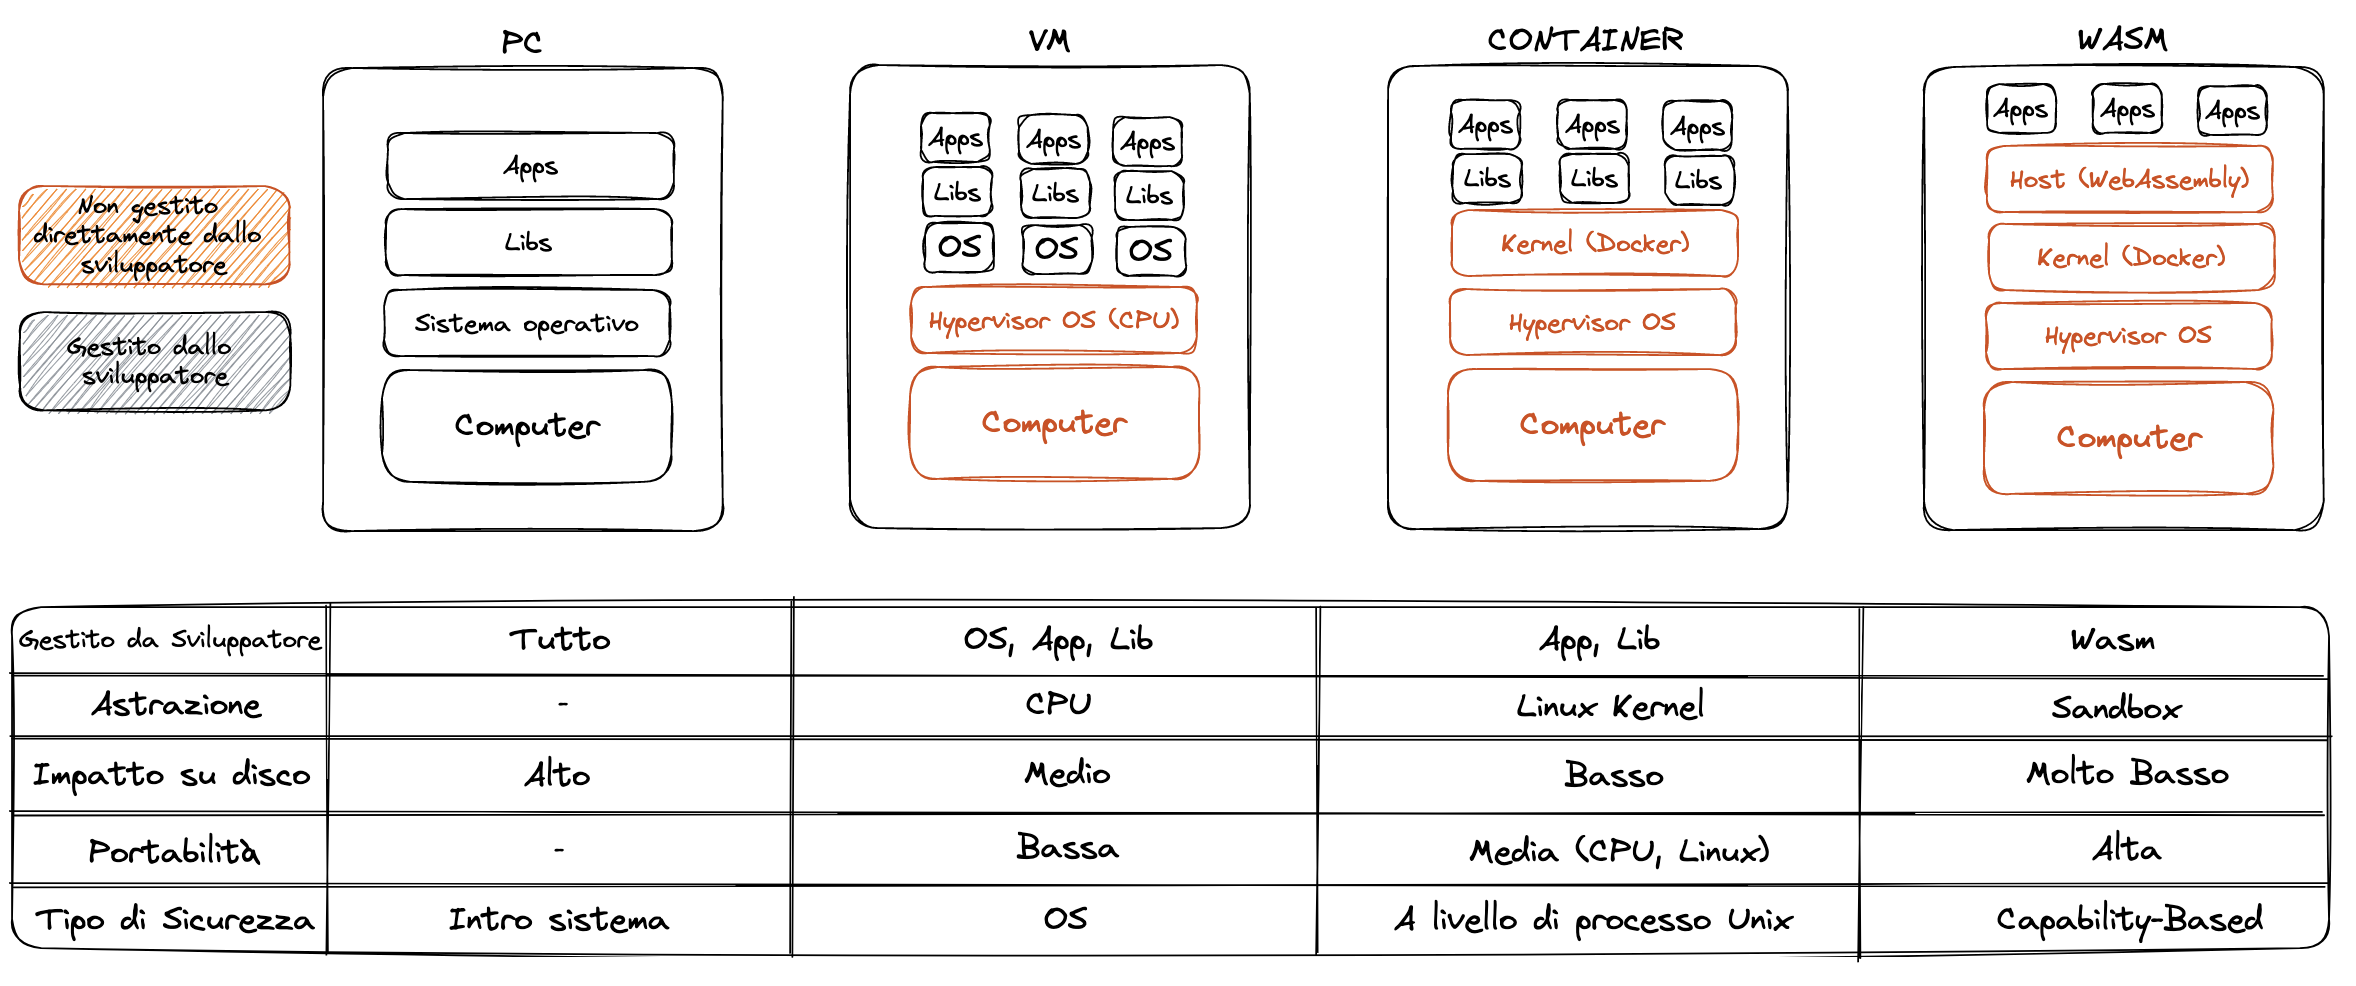
\includegraphics[width=15cm]{./chapters/1.introduction/images/7.wasi_cloud_lightweight.png}
    \label{wasi_wasi_cloud}
    \caption{Evoluzione del cloud computing}
\end{figure}

\begin{quote}
    If WASM+WASI existed in 2008, we wouldn't have needed to create Docker. That's how important it is. Webassembly on
    the server is the future of computing. A standardized system interface was the missing link. Let's hope WASI is up
    to the task! \\
    \textit{Solomon Hykes - Former Docker
    Founder}\footnote{\url{https://twitter.com/solomonstre/status/1111004913222324225}}
\end{quote}

Significa che Wasm rimpiazzerà completamente docker? No, ma è un'ulteriore tecnologia che si aggiunge a quelle già
esistenti, con i propri punti di forza e di debolezza.
\begin{quote}
    "So will wasm replace Docker?" No, but imagine a future where Docker runs linux containers, windows containers and
    wasm containers side by side. Over time wasm might become the most popular container type. Docker will love them all
    equally, and run it all :) \\
    \textit{Solomon Hykes - Former Docker
    Founder}\footnote{\url{https://twitter.com/solomonstre/status/1111113329647325185}}
\end{quote}
